%!TEX root = main.tex

\begin{figure}[!ht]
	\centering
	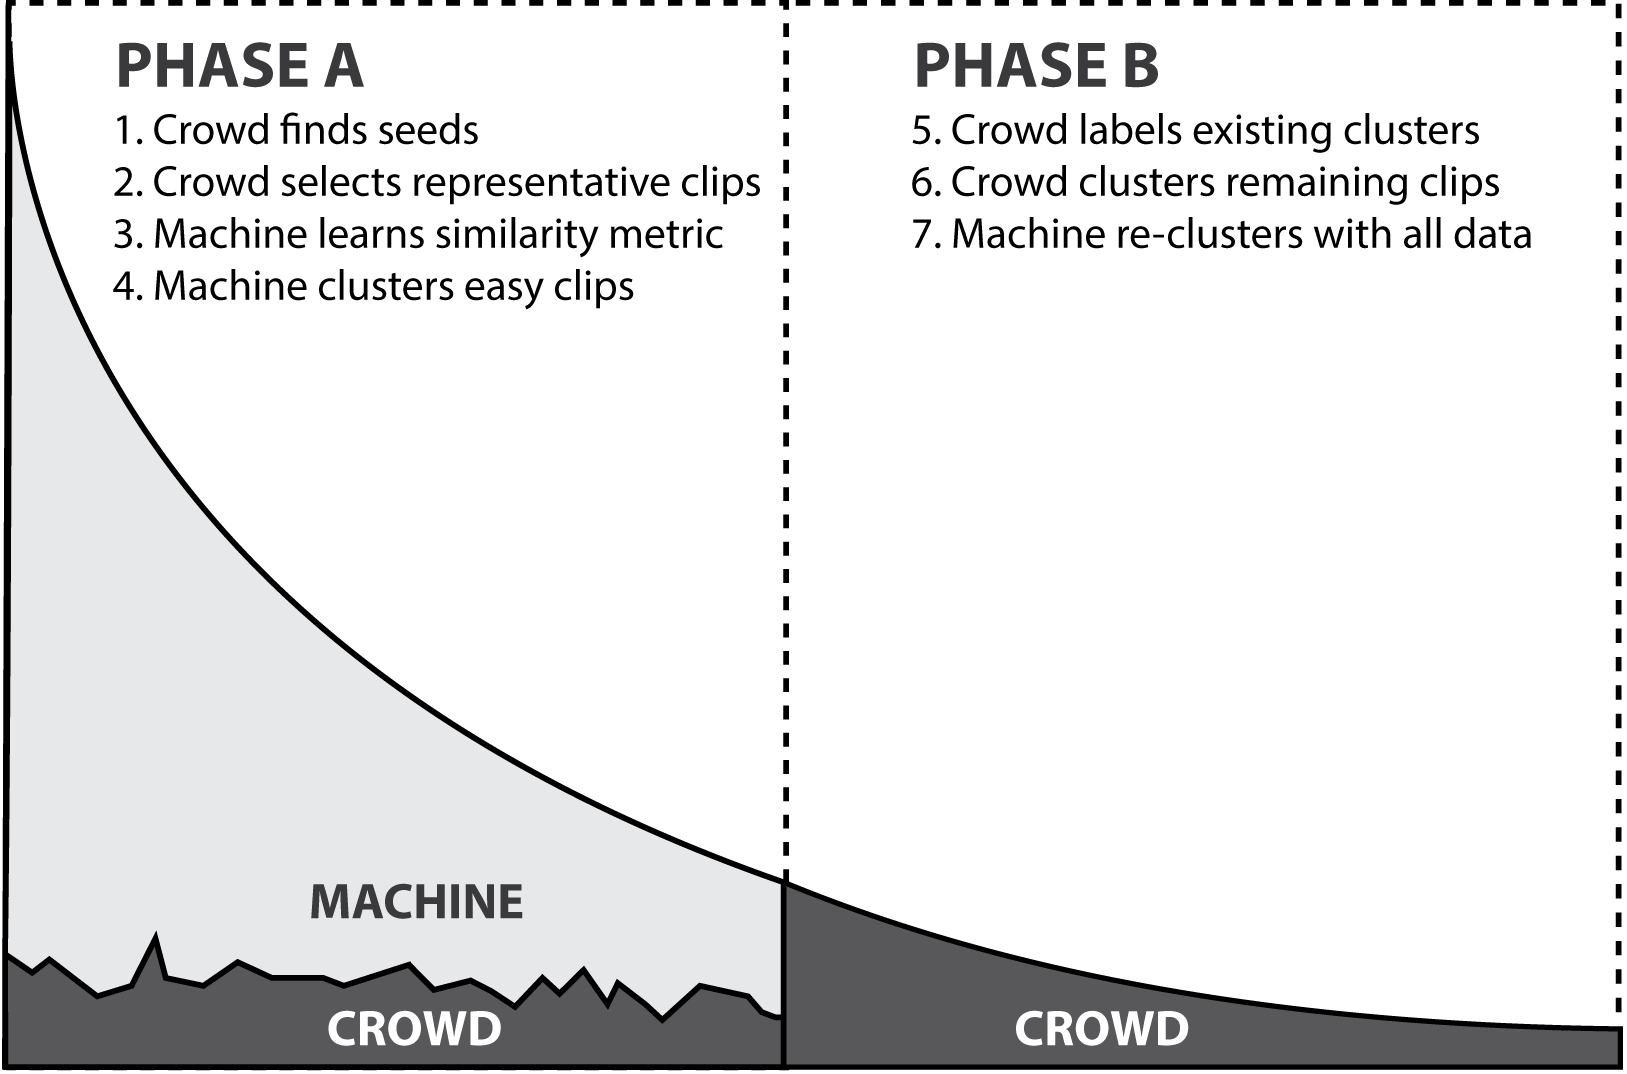
\includegraphics[width=0.6\columnwidth]{Chapters/Alloy/images/alloy_overview_01.png}
%	\caption{First, we use the crowd for creating labels and select features to
%		train a machine learning model. Then, the trained model clusters a
%		large part of the input data.  Finally, the crowd takesover again to
%		refine the output from the machine to produce the final result.}
	\caption[A conceptual overview of the Alloy system.]{
		A conceptual overview of the system. In the first phase, crowd workers identify
		seed clips to train a machine learning model, which is used to classify
		the ``head'' of the distribution. In the second phase, crowd workers classify
		the more difficult items in the ``tail''. A machine learning backbone provides
		a consistent way to connect worker judgments in different phases.
	}
	\label{fig:workflow}
\end{figure}

% - Clustering unstructured information is important, but current machine algorithms have problems understanding deeper semantics of rich textual data. 
% - Recent research has begun to ..., <give examples of current work's success> However, <move examples from related work>.

Clustering, or pulling out the patterns or themes among documents, is a fundamental way of organizing information and is widely applicable to contexts ranging from web search (clustering pages) to academic research (clustering articles) to consumer decision making (clustering product reviews) \cite{jain1999data}.  
For example, a researcher may try to pull out the key research topics in a field for a literature review, or a Wikipedia editor may try to understand the common topics of discussion about a page in order to avoid or address previous conflicts. Doing so involves complex cognitive processing requiring an understanding of how concepts are related to each other and learning the meaningful differences among them \cite{Bellman:2003:DP:862270,kriegel2009clustering,medin1978context}. 

Computational tools such as machine learning have made great strides in automating the clustering process \cite{blei2003latent,chuang2012termite,chaney2012visualizing}. However, a lack of semantic understanding to recognize the important differences between clusters leaves the difficult task of identifying meaningful concepts to the human analyst \cite{chuang2012interpretation}. This reflects an inherent advantage for humans over machines for the complex problem of understanding unstructured data beyond merely measuring surface similarity, and a corresponding opportunity for research in combining human and computational judgments to process complex information \cite{fails2003interactive, Kulesza:2014:SLF:2611247.2557238, hu2014interactive}.

One such promising avenue of research harnesses the power of crowds to identify categories and cluster rich textual data. Crowdsourcing approaches such as Cascade, Deluge, and Crowd Synthesis \cite{chilton2013cascade,bragg2013crowdsourcing,andre2014crowd} have demonstrated the power of splitting up rich, complex datasets into small chunks which can be distributed across many human coders. However, all of these approaches must grapple with a fundamental problem: since each human coder is seeing only a small part of the whole dataset, a lack of global context can lead to incoherent results.  For example, if the items sampled are too similar, the worker might create overly fine-grained clusters. On the other hand, if the items sampled are too dissimilar, the worker might create overly broad clusters. Clusters found in many worker segmentation sets may give rise to redundant clusters, while clusters whose items are sparsely split among segmentation sets may never be realized at all. As an example, \cite{andre2014crowd} cite redundancies in Cascade's top level clusters having both ``green'' and ``seafoam green'', ``blue" and ``aqua'', as well as the encompassing category of ``pastels''. While Crowd Synthesis used an iterative approach to address these redundancy problems, it trades this off with lowered robustness as issues with early workers' categories can cascade throughout subsequent workers' judgments. This suggests the design space of approaches for crowd clustering may be being critically limited by the assumption of splitting up the dataset into small, fixed pieces that prevent workers from gaining a more global context.

Another challenge with current crowd clustering approaches is that using human judgments to label each piece of data is costly and inefficient. Deluge addresses some issues with efficiency, improving on Cascade by reducing the number of human judgments elicited as the rate of new category generation slows \cite{chilton2013cascade}. However, these crowd clustering algorithms still require human judgments for every item, which is costly. In the real world data often follows a long-tailed distribution in which much of the data is captured by a small number of categories in the head of the distribution \cite{white2007studying}. For such data in which many items in the head of the distribution are likely to be highly similar, once humans have identified the meaningful categories and representative examples it would be more efficient if a machine could classify the remaining items in those categories. A danger with such an approach is that the sparse categories in the tail of the distribution with few examples may be difficult to train a machine to recognize, and so human judgments may have another important role in ``cleaning up'' low frequency categories.

%Past work also explored ways to combine expert workers and computation for categorizing unstructured textual information using interactive interfaces \cite{huang2006text,settles2011closing}.
%Both studies showed that using one expert worker to identify a small set of informative keywords can significantly improve the results of machine clustering on the 20 newsgroup dataset, where each category has similar number of articles.
%However, it is also common for a collection of information to be not evenly distributed across topics, but instead follow a highly skewed distribution \cite{white2007studying}. In such cases, statistical based algorithms may perform well on the typical cases in prominent topics of the dataset, but fail to capture the edge cases and the smaller categories. 
%Intuitively, it could be greatly beneficial to use human judgements again to clean up the output, covering cases that are difficult for the machines but relatively simple for people.


%Such advantage is partly based on a good global understanding of the information at hand, which either comes from prior knowledge and/or comprehending the entire dataset for expert workers.
%However, this creates challenges for system designers due to the distributed nature of crowdsourcing \cite{Kittur:2013:FCW:2441776.2441923}, namely the lack of domain knowledge of the workers and the difficulty of providing enough global information in a microtask for finding good categories.
%Since it is infeasible to ask crowdworkers to read all items in the dataset, current work simply employs crowdworkers to process arbitrarily parts of the dataset \cite{chilton2013cascade,andre2014crowd}. 
%This lack of global context can lead to incoherent results, because different workers are creating clusters based on different small pieces of the puzzle. For example, if the items sampled are too similar, the worker might create overly fine-grained clusters. On the other hand, if the items sampled are too dissimilar, the worker might create overly broad clusters. 
%In general, most current systems provide context by showing a small sample of items, hoping that it captures the distribution of information in the larger dataset. 

%People have been developing machine learning algorithms to cluster unstructured rich textual data using similarity measurements based on surface features. However, without deeper semantic understanding of the information at hand, it can be difficult for machines to distinguish which features embody useful categories.
% For example, \emph{sunlight} and \emph{lights} are potentially good features for the first text clip in Figure~3 if other items in the dataset are about ways to better grow tomatoes, but not so if other items are about the seeding of various plants. 
%For example, \emph{liquid water} is potentially a good feature for the second text clip in Figure~3 if other items in the dataset are about key factors of supporting life on a planet, but not so if other items are about the various roadmaps of NASA. 
%Human intellect, on the other hand, is readily able to infer meaningful categories from complex data given enough context  \cite{Bellman:2003:DP:862270,kriegel2009clustering,medin1978context}. This gives crowds an inherent advantage over machines for the complex problem of understanding unstructured data beyond merely measuring surface similarities, and a corresponding opportunity for research in combining crowds and computation to cluster complex information.



% 
% \joseph{new}
% % moded from the info-seeking framing
% Whether researchers, shoppers, students, or voters, a common challenge is
% synthesizing information gathered from multiple sources into
% meaningful and useful categories
% to gain a bigger picture in order to 
% identify the core topics,
% such as specs for a new product, ways to
% unclog a drain, organizing research papers into conference session, or the key issues
% involved in an election. 
% For example, an individual searching for health information may have
% to go to over a dozen web sites in order to get a complete picture of a domain
% \cite{bhavnani2005difficult}. While doing so information seekers aim to
% determine the common themes and the distribution of information across those
% themes, eventually trying to decide which information is important and which sources to
% trust \cite{kittur2014standing}.  This represents a substantial cognitive
% challenge and a corresponding opportunity for research in better supporting
% individuals engaged in these tasks. 

% dont draw attention to scaling
%In this paper, we explore an alternative approach of an ad hoc, crowd-driven
%method for finding structures and organizing %datasets with less than a few thousand items.



% 1. keywords can help machines get much better results
% 2. skew distribution
% 3. machines output still needs human clean up 




% A key difference from previous work on crowd clustering is our two-stage model
% of clustering.
% %There is a conflict between providing sufficient context
% %for identifying categories in a skewed distribution and the limited context capacity of
% %microtasks that are suitable for posting to online crowdsourcing marketplaces such as Amazon Mechanical Turk. Further, i

% In such cases the head of the topic distribution
% contains a disproportionate number of clips, and once a human has labeled a few
% of these clips it is inefficient to continue using human labor to finish
% labeling them as automated methods can do a reasonably good job.  Conversely,
% the tail of the topic distribution contains topics with few clips,
% and expending resources to train a machine learning algorithm to
% identify these sparse topics is less advantageous, while it is comparatively
% easy for humans to classify these clips.

% Previous crowdsourcing research has shown success in using the crowds to capture uncommon cases in a long tailed distribution to improve inline answers in Web search engines \cite{Bernstein:2012:DAS:2207676.2207710}.



% 
% , it can lead to problems
% enforcing global constraints such as redundant or overly similar
% categories, categories at the wrong level of abstraction due to lack
% of context, categories that do not represent the distribution of
% information faithfully because of sampling issues, or simply inadequate categories
% because of worker motivation or expertise issues. 
%
% dont draw attention to scaling
% Furthermore, hiring workers
% incurs monetary costs and thus can have issues scaling to large amounts
% of data compared to computational approaches. 
%
% old framing for "the but"
% Existing crowd clustering approaches have addressed some of these
% challenges, but often with significant trade-offs. For example, 
% methods that are robust against a few poor judgements often fail to enforce global
% constraints, leading to overlapping, incoherent, or duplicated categories. On the other hand,
% methods that focus on producing
% coherent results by providing global view to the crowds are often vulnerable to a few
% poor judgements in early stages cascading through the workflow
% \cite{chilton2013cascade,andre2014crowd}.
%
% 
% This paper describes Alloy, a crowd-based short text clustering workflow that uses a \emph{sample-and-search} process to build up workers’ mental models with context beyond showing multiple arbitrary items.
% We believe this is a new way to support global context for crowd clustering.

% In addition, we introduce a \emph{cast-and-gather} framework that allows Alloy to cast out various types of microtasks for different types of human judgements, and gathers them using a machine learning backbone. With this framework, Alloy 
% incrementally cluster the datasets in a two-phase approach: First, workers actively request for context by repeatedly sampling random items and searching for similar items in the entire dataset while building up their mental model of the global context. Based their labels, a machine classifier then clusters unlabeled items with high confidence, capturing the prominent categories (the head of the distribution). Then, crowdworkers switch roles from trainers to cleaners, capturing smaller clusters and items that are difficult for the machine classifier (the tail of the distribution).

This chapter describes Alloy, a hybrid approach to text clustering that combines the richness of human semantic judgments with the power of machine algorithms. Alloy improves on previous crowd clustering approaches in two ways. First, it supports better global context through a new ``\emph{sample and search}'' crowd pattern which changes the crowd's task from classifying a fixed subset of items to actively sampling and querying the entire dataset. Second, it improves efficiency using initial crowd judgments to help a machine learning algorithm cluster high-confidence unlabeled items in the head of the distribution (prominent categories), and then uses later crowd judgments to improve the quality of machine clustering by covering the tail of the distribution (edge cases and smaller categories). 
To achieve these benefits, Alloy introduces a novel modular approach we call ``\emph{cast and gather}'' which employs a machine learning backbone to stitch together different types of crowd judgment tasks. While we provide a particular instantiation of the cast and gather approach here (with a hierarchical clustering backbone which gathers three types of crowd tasks, or ``casts''), the general framework for modularizing multiple types of human judgments with a common machine-based backbone may inspire application to other contexts as well.


% old framing for the therefore
% 
% We introduce Alloy,
% a new approach to structure complex information by identifying meaningful clusters of short text
% with crowds and computation.
% Alloy is based on the intuition that we
% can employ the crowd to act first as a guide, highlighting the high-level
% structure of a domain as training for a machine learning model; then, after
% the algorithm has classified instances that are easy for it to
% categorize, the crowd can further clean up the results by categorizing the
% remaining instances that proved more difficult. Different from many of the previous
% approaches which gather small and independent human judgements for all
% instances and stitch them together to infer concepts,
% we use a machine learning model to scale crowd judgements to cover unlabeled instances.  
% By using a two phase approach, we try to compensate for the shortcomings of crowdsourcing (e.g., lack of context,noise) and machine learning (e.g., sparse data, lack of semantic understanding) by utilizing techniques from both fields. 
% We focus on providing rich context
% to crowdworkers and transferring context between workers in different phases with a machine backbone algorithm.
% Using this approach we aim to enforce global constraints while
% also leveraging machine learning to increase scalability and to protect against
% poor worker input.

\subsection{Related Work}

%\niki{want to start with a paragraph that sets up the importance of clustering
%    itself and gets to the crowd framing faster. Like the paragraph two down
%    from here. I'd put these two paragraphs later in the intro or in a related
%    work section. Remember that an AC will probably skim the first couple
%    paragraphs to decide who to recruit as reviewers. }

Document and short text classification are well researched topics in natural
language processing and machine learning. With enough labeled training data,
state-of-the-art algorithms can often produce good results that are useful
in real world applications. Yet building such systems often requires expert
analysis of specific datasets both to manually design an organization scheme and
to manually label a large set of documents as training data. Unsupervised approaches, 
or clustering,
aim to discover structures on-demand and without expert preparation
\cite{jain1988algorithms,hartigan1975clustering,steinbach2000comparison}.
While these
data mining approaches may discover dimensions (features) that provide a good
separation of the dataset, the inferred categories can be difficult for a human
to interpret, and many of them may not capture the most meaningful or useful
structure in a domain due to high dimensionality or sparseness in the word vector space 
\cite{Bellman:2003:DP:862270,kriegel2009clustering}.
To deal with these issues, researchers have explored ways to automatically
discover topical keywords that can help identify useful categories in unstructured data
such as TF-IDF, latent semanic analysis, and latent
Dirichlet allocation \cite{manning2008introduction,Jones72astatistical,deerwester1990indexing,blei2003latent}.
However, even with these improvements, automatic methods often still
perform poorly, especially when the number of document is small, the lengths
of the documents are short, or when the information is sparse.


% 
% People have been utilizing different machine algorithms to organize 
% huge datasets
% such as research paper archives or newsgroup articles. Unsupervised methods, such as
% Latent Dirichlet Allocation \cite{blei2003latent}, rely on tens of thousands of articles for discovering
% salient features. However, there are also many cases where the amount of
% information at hand is less than sufficient for such methods. For example, during online exploratory 
% information seeking, people typically go through dozens of sources.
% When organizing sessions for a conference, there are typically a few hundred
% accepted papers. On the other hand, supervised methods
% can organize datasets of different scales once a classifier is trained,
% but it requires prior expert knowledge
% to define classes, precompile a large dataset, and create labels 
% for training. This process, besides being expensive in time and expertise, can also be
% difficult to adapt to a different context. For example, the classes designed for a CHI paper
% classifier may not be fine-grained enough to organize papers in a more focused conference
% such as CSCW. 



More recently, researchers have begun to use crowds to organize datasets without predefined categories.
Cascade \cite{chilton2013cascade}
attempts to address abstraction and sampling problems by first having
multiple workers generate categories for each item and then later having
workers choose between them. By providing limited context to each worker (8 items or 1 item with 5 categories), it suffers from 
categories that can have varying levels of specificity. As a follow up study, Deluge \cite{bragg2013crowdsourcing} produces
comparable results, but with significantly lower cost by optimizing
its workflow using machine algorithms. In another line of research, Crowd Synthesis \cite{andre2014crowd} showed that providing more context by simply showing more items can lead to significant better categories, suggesting that global context is one of the key elements for crowd clustering algorithms.
In general, most current systems provide context by showing a small sample of items, hoping that they captures the distribution of information in the larger dataset. 
We propose an alternative approach that builds up workers' mental models by asking them to repeatedly sample for new items, identify discriminative keywords, and search the dataset for similar items, taking advantage of people's capacity of information foraging \cite{pirolli1999information}.

% Furthermore, a dataset can be organized with very
% different categories for different purposes (e.g., author perspectives vs
% topics), and it is often difficult for unsupervised methods to
% take into account the context for organizing documents into conceptual groups.
% For these reasons, there seem to be room for exploring methods that make use of 
% both the crowd and machine to not just label documents with predefined classes
% for training supervised models, but also to identify the innate structure of
% the dataset that fits a given context.


% the info-seeking framing
% Whether researchers, shoppers, students, or voters, a common challenge is
% synthesizing information encountered from diverse online sources into
% meaningful and useful categories, such as specs for a new product, ways to
% unclog a drain, the factors that make a planet habitable, or the key issues
% involved in an election. Important information can be scattered across many
% sources; for example, an individual searching for health information may have
% to go to over a dozen web sites in order to get a complete picture of a domain
% \cite{bhavnani2005difficult}. While doing so information seekers aim to
% determine the common themes and the distribution of information across those
% themes, eventually trying to decide which information is important and which sources to
% trust \cite{kittur2014standing}.  This represents a substantial cognitive
% challenge and a corresponding opportunity for research in better supporting
% individuals engaged in these tasks. To provide a sense of the the magnitude of
% this opportunity, estimates put the amount of time spent on such complex
% sensemaking tasks at around 70 billion hours per year in the U.S. alone, or
% around 30\% of the time people spend online
% \cite{kellar2007field,Fisher:2012:DSI:2207676.2207711}.


A complementary set of approaches to crowd clustering research has focused on
addressing the scaling problem through computation, applying approaches such as
partial clustering \cite{yi2012crowdclustering}, learning similarity metrics
through triad-wise comparisons \cite{tamuz2011adaptively}, or using matrix
completion to reduce the number of labels needed from
workers \cite{yi2012semi}. 
While these approaches have shown to be powerful on simple
information such as images or travel tips, synthesizing more complex
information can be difficult without providing novice crowdworkers with richer
context or opportunities to deeply process the data. 

%
% Novices are especially
% susceptible to creating superficial categories, using too much or too little
% abstraction, or failing to notice a category entirely
% \cite{chilton2013cascade,andre2014crowd}.


% (remove b/c space)
% Some of the core challenges this approach addresses include:
% 
% \begin{itemize}
% \item \emph{Lack of expertise}. Typical crowdworkers do not have the domain expertise.
% 	Without enough context to help them build some background knowledge, they
% 	may cluster the data into superficial classes based on the surface patterns
% 	rather than deeper understanding of the information.  Furthermore, without
% 	enough context to provide some idea of the information landscape, they may
% 	also create classes that are too general and ill-organized.
% \item \emph{Disagreement}. Crowdworkers may create different and conflicting
% 	feedback, because they understand the same dataset from different
% 	angles, thus creating clusters based on different features.
% 	Further, even if they are working from similar viewpoints, they
% 	may create clusters at different levels of abstraction.
% \item \emph{Capacity}. The two challenges above can potentially be ameliorated
% 	by providing more contextual information to the crowdworkers. However, it
% 	is difficult to provide a large amount of information to build up their
% 	mental model, while keeping the microtasks manageable. In our case, it
% 	would be unreasonable to present the workers with the complete raw corpus,
% 	due to the size of the datasets.
% \item \emph{Aggregation}. Due to the \emph{capacity} challenge, each worker may
% 	only be working on a portion of the dataset. However, unlike tasks that
% 	label independent items, e.g., classify an image, items in the clustering
% 	task are not independent.  If each crowd worker only worked on a small set
% 	of the data, how do we put their independent judgements together to form a
% 	complete answer?
% \end{itemize}

% Clustering data by analyzing the underlying structures to discover abstract
% themes and concepts is a common and important procedure in a wide variety of
% tasks ranging from human learning and decision making to market research and
% recommender systems. For example, grouping accepted papers to form conference
% sessions, segmenting markets to identify the target customers, and grouping
% similar product reviews to provide a quick overview.  Whether performed by a
% person or an algorithm, the essence of such processes involves identifying the
% salient features for a given context, recognizing similar items based on the
% identified features, and discovering abstract classes (concepts) to form
% clusters. The same dataset may also be clustered differently under different
% contexts. For example, libraries may organize books based on different topics,
% while online bookstores may organize their products based on the characteristic of
% their previous and potential buyers.  However, even for humans, this process
% can be time-consuming and cognitively taxing, because it requires a global view
% of the data and a deep understanding of the context and domain to determine the
% importance of different features and arrive at a coherent grouping of meaningful
% clusters.


% Researchers have also begun to explore the use of the crowd to discover partitions
% in different types of datasets. Earlier work focused on creating labeled
% datasets for supervised or semisupervised training
% \cite{Raykar:2010:LC:1756006.1859894} and clustering image datasets
% \cite{yi2012crowdclustering,tamuz2011adaptively}.  More recently, research
% efforts have also been made in clustering complex information represented in
% text  \cite{yi2012crowdclustering,andre2013community,andre2014crowd}.

% weak sauce
% Past work has dealt with general datasets that utilize crowdworkers' everyday
% knowledge (colors, general travel tips, images of everyday objects) or domain
% specific datasets (Wikipedia ``barnstar'' awards). Unlike previous approaches,
% we employ a multi-phase approach that accounts for the weaknesses of humans
% (e.g., scaling) and machines (e.g., understanding context). Specifically,  the
% crowd first learns the context of an information space, then provides feedback
% to train a machine learning algorithm for recognizing that same context. We then
% leverage the algorithm to classify many instances on the fly, and return to the
% crowd to verify and fix the machine's clustering.

% Niki's comment
% Why are we working with such clips?  I.e., why is it important to be able to
% cluster web clips? (e.g., 30\% of the time people spend online is about complex
% information seeking where people are trying to pull structure out of and
% synthesize pieces of information from across many web pages). Generally, I
% think this whole paragraph could be moved up to the beginning (right after your
% first paragraph) and used to frame the problem we are working on.  
% Niki's comment2
% we focus on the problem of clustering snippets of information from the web.
% This task is a critical part of a larger research program aiming to synthesize
% information from diverse web pages into a cohesive whole, and could help
% address the issue of information scatter on the web (Bhavnani cite).
% [actually, probably want to move this to later]

% that we can work on the same data but provide a new way of combining crowds
% and computation to make up for the weaknesses of each approach?
% ** how?
% Add a bridging sentence that gives the intuition of the approach.  E.g.,``The
% key idea is that we break the problem into two phases; in the first phase we
% use the crowd to train a machine classifier to cluster the majority of the
% dataset, and in the second phase we use the crowd to manually classify those
% data that were not easily clustered by the machine'' (or something like that)

% In this paper, we present an empirical study of a two-phase approach that makes
% use of both human computation and text processing algorithms to tackle the
% problem of clustering complex information.  The key idea is that we break the
% problem into two phases; first, we use the crowd to train a machine classifier
% to cluster the majority of the dataset, then, we use the crowd to manually
% classify those that were not easily clustered by the machine. More
% specifically, in Phase A, we partially cluster the input dataset at the level
% of abstraction that is based on the clustering agreement and feature (keywords)
% extraction from a number of crowdworkers collected via a partial clustering interface. A
% classifier is trained on-the-fly using the feedback from the crowdworkers to
% measure the pairwise similarity of the items in the dataset, and the
% agglomerative clustering algorithm is performed to create intermediate clusters
% that the majority workers agreed upon. In this phase, the workers only work
% with a portion of the entire dataset, but create feature dimensions that are
% applicable to all items in the datasets.  In Phase B, the partially clustered
% dataset from the previous phase is presented to a number of crowdworkers, and global
% clustering agreement is collected via a global clustering interface to form
% the final output. In this phase, the workers have access to the entire dataset,
% in which a large portion is already clustered. By using this two phase
% approach, the algorithm can effectively create clusters from complex datasets at
% appropriate level of abstraction, even for datasets that are too large to be presented
% in full to a single crowdworker.

% Major contributions of this work include:
% \begin{enumerate}
% 	\item We explore the possibility of using novice crowdworkers not only to
% 		create answer labels, but also to extract meaningful feature
% 		dimensions through an interactive search process and train an SVM model
% 		to measure the similarity between items.
% 	\item We propose a method that is robust even if a few workers provided
% 		poorly organized results. Where as in previous systems, a single
% 		crowdworker labeling every item with a general topic (e.g.,
% 		\emph{solutions} or \emph{tips}) can have devistating effects on the
% 		quality of the feedback from subsequent crowdworkers.
% 	\item We use a two-phase process that makes use of both statistical models
% 		and aggregates agreements among crowdworkers to produce clusters at an
% 		appropriate level of abstraction for the given context.
% 	\item Previous work are mostly evaluated on clean datasets, where all items
% 		are valid, while we work with noisy datasets of short webclips gathered
% 		by crowdworkers, showing how the process can be robust to even 30\% bad
% 		input.
% % Niki: Why is this a contribution?  Maybe because we are sharing the gold standard data?
% % 	\item In addition to reviewing the clustering results for evaluation, we
% % 		created gold standard answers for complex datasets. We also present
% % 		inter-annotator agreements for each collections, and discuss the innate
% % 		properties of each corpus and how they effect the clustering process.
% \end{enumerate}


% ^^^^^ FINAL ANSWER AREA ^^^^^

% The rest of the paper is organized as follows: In the next section, we review
% previous works that are most relevant to our research. We then describe in
% detail the two-phase produces of the proposed method in the Method Section. We
% also explain the experimental settings and the datasets.  Finally, we show the
% empirical results of our experiments, and conclude in the last section.


